First, in this section, we formalize a stream processing engine based on Chandy-Lamport distributed system definition. This model is more low-level than the model introduced in~\ref{fs-formalism} since it covers messaging between processes. Finally, we define the substream management problem based on the notions from the proposed model.

\begin{table}[!b]
\begin {center}
    \caption{Notations used throughout the chapter}
    \footnotesize
    \begin{tabular}{l|p{5cm}}
        \hline
        $p$ & Process (node in a physical execution graph) \\ 
        \hline
        $I_p$, $O_p$ & input and output channels of a process $p$ \\ 
        \hline
        $func_p(U, M)$ & User-defined operator run by process $p$. It receives current operator state $U$ and an incoming message $M$ \\ 
        \hline
        $\Pi$ & The set of all processes  \\
        \hline
        $K$ & Number of substreams (can be unlimited if substreams are regularly created) \\
        \hline
        $c$ & A network channel between processes  \\
        \hline
        $\mathcal{E}$ & The set of all network channels  \\
        \hline
        $s_p = U_p \cup B_p$ & State of the process $p$ consists of a mailbox $B_p$ and a state $U_p$ of $func_p$ \\
        \hline
        $mbc_{p}$ & Mailbox controller of a process $p$ \\
        \hline
        $e_{p}$ & Event of a process $p$ \\
        \hline
        $Pred(e)$ & Propositional formula defined on events \\
        \hline
        $pred(M)$ & Propositional formula defined on messages\\
        \hline
        $t(M)$ & Coarse time label \\
    \end{tabular}
    \label{notations-substreams}
\end {center}
\end{table}

\subsection{Distributed Streaming Model}
\label{fs-acker-spe-model}

Typically, distributed stream processing engines are shared-nothing runtimes that continuously ingest input elements, transform them according to a logical dataflow graph, and deliver output elements. The logical dataflow graph consists of user-defined operators. Operators are functions of a single input data element that produce output data elements. Operators can be stateless or stateful: output elements may depend on the current state. An SPE maps a logical graph to a physical (distributed) graph on deployment. Commonly, a single logical operator can be deployed on multiple computational nodes. Further, we denote physical instances of logical operators as {\em processes}.

We can describe a deployed physical graph as a distributed system in Chandy-Lamport model~\cite{Chandy:1985:DSD:214451.214456, carbone2018scalable}. In this model, the authors introduce \textit{events} that allow observing the entire system's state. This approach allows defining system-wide guarantees: in the original paper, authors used it to introduce the notion of {\em consistent state}. We use this approach for the definition of a substream management problem.

Following the notation from~\cite{Chandy:1985:DSD:214451.214456, carbone2018scalable}, one can observe a distributed system with events. 

\begin{definition}[Event]
An event is a tuple of 5 elements $e = (p, s, s', c, M)$, where $p$ is one of the deployed processes, $s$ and $s'$ are the state of the process before and after processing, $c$ is one of network FIFO channels that connect processes, and $M$ is a message generated during processing.
\end{definition}

The generated event $M$ comes to a channel state $C$ until the destination process receives it. Processes and channels form a physical graph of the system $G=\{\Pi,\mathcal{E}\}$. We denote all input channels as $I_p$ and output channels as $O_p$.

In a stream processing engine, we need to specify a process $p$ to reflect the nature of SPE. 

\begin{definition}[Process]
A process in an SPE is an actor consisting of {\em business logic handler} (BLH) and {\em mailbox controller} (MBC). The first block encapsulates a user-defined operator. The user-defined operator does not directly communicate with other processes in the system. Instead, it receives and generates {\em messages} -- data elements tagged by their source and destination. The mailbox controller handles further delivery of these messages along the communication channels and preserves the order of message generation.
\end{definition}

Figure~\ref{fig:spe_process} illustrates the scheme of a process. This system layout is not new and is widely used in practice (Akka, YDB, Millwheel, etc.).

\begin{figure}[t]
  \centering
  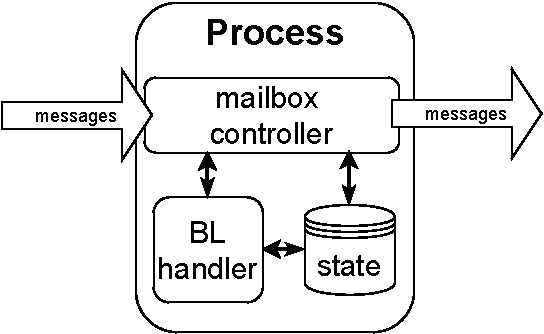
\includegraphics[width=0.6\textwidth]{Chapters/SubstreamConsistency/pics/process-scheme.pdf}
  \caption{Structure of the SPE process}
  \label{fig:spe_process}
\end{figure}

\subsection{Stream Processing Events}

When a process receives a message, the mailbox controller puts it into a particular segment of the process state ({\em mailbox} $B_p$). The business logic handler gets a message provided by MBC and triggers a user-defined operator. The user-defined operator processes the data element that the message contains and generates an arbitrary number of outgoing messages. BLH puts generated messages back in a mailbox. MBC sends outgoing messages along communication channels to destination processes. All mailbox controller operations respect the order of messages in the mailbox. If a user-defined operator has a state $U_p$, the joined process state will consist of the mailbox and this state $s=U_p \cup B_p$. In the Chandy-Lamport paradigm, this algorithm produces the following events within a process:
\begin{itemize}
    \item Communication events: $\langle recv, p, M\rangle$, $\langle send, p, M \rangle$ -- these events are handled by mailbox controller
    \item Processing of an incoming message $\langle proc, p, M, M' \rangle$
\end{itemize}

Let us translate these events into 5-tuple language. Communication events move a message between the communication channel and the mailbox section of the state:

\begin{equation}
\langle recv, p, M\rangle = (p, s_p, s'_p = U_p \cup \left(B_p \cup \{M\}\right), c_{qp}, M)
\end{equation}

\begin{equation}
\langle send, p, M \rangle = (p, s_p, s'_p = U_p \cup \left(B_p\setminus\{M\}\right), c_{p, dst(M)}, M)
\end{equation}

This function translates a destination of an element from logical dataflow graph nodes to physical communication channels between processes. Note that we need to be able to get a destination process directly from the message $dst(M)$. A practical case of this abstraction is a sharding scheme for some key: a user-defined procedure emits an event for some key, and a system is responsible for finding a proper physical channel to deliver this message.

Incoming message processing does not influence the communication channels and only ingest results of a message processing $(U', M') = func_p(U, M)$:
\begin{equation}
    \langle proc, p, M, M' \rangle = (p, s_p, s'_p = U'_p \cup \left(B_p \setminus \{M\} \cup M' \right) , \emptyset, \emptyset)
\end{equation}

Note that in this case, $M'$ may contain multiple messages. Following the Chandy-Lamport model, we assume processes are single-threaded, so within the specific process $p$, all events are ordered by a local causal order relation $<_p$: $e^{0}_p,e^{1}_p,\ldots,e^{i}_p,\ldots$. Please note that each process has its own local causal order relation, so we do not assume any total order among events from different processes. This model is indeed practical, e.g., implemented in actor-based systems.

\subsection{Substream Lifespan}

We want to get a substream's first and last element for each process. One can easily find the first one when it emerges, but verification that there will be no more events of a substream could be problematic. The strict substream termination guarantee consists of two parts: the source must promise that no more messages from the substream may emerge, and the system must ensure it contains no substream messages. The first task requires a contract with a particular data source and is thus out of scope for this chapter, though it is discussed in relevant literature~\cite{awad2019adaptive}. Instead, we focus on the second task; this is challenging due to distributed nature of the system and the absence of a standard message lifetime limit. This difficulty increases with the introduction of cycles into dataflow. Crucially, processes are not isolated, and substream messages can move from one process to another. That is why we need to observe all in-flight messages in the system.

\begin{definition}[Substream]
All events in a system satisfying a propositional formula $Pred(e)$ form a substream.
\end{definition}

We have to use system events as they are ordered inside each process and can define a border of a substream. Sometimes it is more practical to induce this predicate to messages ($pred(M)$) involved in processing: $Pred(e) = (e = \langle proc, p, M, M'\rangle) \wedge pred(M)$.

We consider substreams with a limited lifespan within a process. We want to know when a substream starts and terminates: 

\begin{equation}
\forall p, \exists t_0^p, t_1^p: \exists e: e_{t_0^p} <_p e <_p e_{t_1^p}, Pred(e) \And \forall e': e_{t_1^p} <_p e', \neg Pred(e') 
\end{equation}

We can boil this formula down: for each process $p$ in the system, there must be two event indices $t_0^p$ for substream start and $t_1^p$ for its termination, such that events satisfying $Pred$ must be between them. 

\begin{definition}[Substream Management Problem]
A substream management problem is to estimate a substream bound for each process. To indicate the bound of a substream for a process, we use a termination event or end-of-substream event:
\begin{equation}
  \langle eoss, p, Pred \rangle = (p, B_p, B_p\cup eoss(Pred), \emptyset, \emptyset)  
\end{equation}
\end{definition}

Some problems require additional properties of the termination events. For example, the state pruning problem does not require any particular properties, while for the state snapshotting problem, the substream management system should detect the exact substream bound. In the following sections, we formalize these properties. 

\subsection{Soft Bound}

Many applications that apply substream management systems do not require any particular properties of termination events. In this case, we denote the guarantee provided by such events as {\em soft bound} because termination events indicate that the substream ended some time ago.

\begin{definition}[Soft bound]
Termination event (end-of-substream) $\langle eoss_{soft}, p, Pred\rangle$ satisfies a soft bound guarantee iff:

\begin{equation}
\forall e, e >_p \langle eoss_{soft}, p, Pred\rangle \Rightarrow \neg Pred(e)
\end{equation}
\end{definition}

Figure~\ref{general_guarantees} illustrates this notion. Terms $a,b,c,d...$ denote ordered processing events of a process $p$. The substream ends after event $c$. Note that there are several other events between the end-of-substream and $c$. If $\langle eoss_{soft}, p, Pred\rangle$ occurs, all subsequent elements do not satisfy the predicate, but it is not necessarily the exact substream ``border''.

\begin{figure}[t]
  \centering
  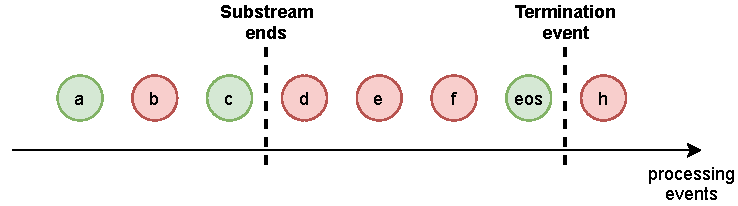
\includegraphics[width=0.80\textwidth]{Chapters/SubstreamConsistency/pics/general-guarantee.pdf}
  \caption{Substream management: soft bound}
  \label{general_guarantees}
\end{figure}

\subsection{Firm Bound}

The guarantee that any new event will not satisfy the predicate is sufficient for many real-life problems, e.g., SPE can initiate process state pruning on such events. However, some problems require a {\em firm bound}: guarantee that the substream ends {\em exactly} after the termination event. 

For example, a commonly used snapshotting protocol~\cite{2015arXiv150608603C, jacques2016consistent} relies on an {\em epoch}. An epoch is a special substream that must be processed atomically. Therefore, the SPE requires the termination event for a given epoch to occur immediately after the last processing event belonging to that epoch. Otherwise, the snapshot can be inconsistent, capturing elements from multiple epochs. The end-of-substream event $\langle eoss_{firm}, p, Pred\rangle$ should satisfy a {\em firm bound } guarantee to support such scenarios.

\begin{definition}[Firm bound]
Termination event (end-of-substream) $\langle eoss_{firm}, p, Pred\rangle$ satisfies a firm bound guarantee iff:

\begin{equation}
\langle eoss_{firm}, p, Pred\rangle = \inf_{<_p} \langle eoss_{soft}, p, Pred\rangle
\end{equation}
\end{definition}

Unlike the soft bound, within the firm guarantee, the first element outside the substream $Pred$ must be ordered after the firm bound event in the process $p$. This position satisfies the first possible soft bound in the events ordering. Figure~\ref{strict_guarantees} illustrates the notion of the firm bound. As in the previous example, terms $a,b,c,d...$ denote ordered processing events of a process $p$. However, in this case, event $\langle eoss_{firm}, p, Pred\rangle$ occurs right after the substream terminates.

\subsection{Consistent Termination Events Order}
Some applications require synchronization between substream termination events and substreams' last elements processing. Among these applications are epoch-based snapshotting methods and techniques for enforcing deterministic processing~\cite{we2018adbis}. For example, snapshots for consecutive epochs can be inconsistent if termination events reordering occurs. Another example is deterministic join~\cite{gulisano2016scalejoin}, which also requires the synchronized order of termination events.

\begin{figure}[t]
  \centering
  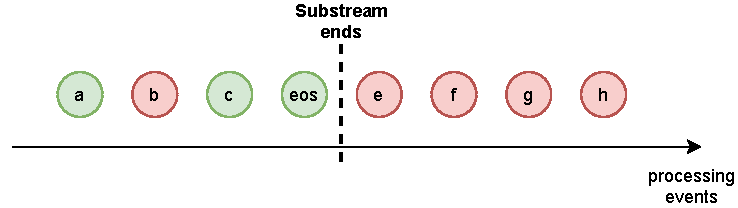
\includegraphics[width=0.80\textwidth]{Chapters/SubstreamConsistency/pics/strict-guarantee.pdf}
  \caption{Substream management: firm bound}
  \label{strict_guarantees}
\end{figure}

Figure~\ref{notifications_reordering} illustrates termination events reordering in the case of the soft bound guarantee. Terms $a,b,c,d...$ denote ordered processing events of a process $p$. Although the substream containing events $a,b$ terminates earlier, the end-of-substream event for this substream occurs after the termination event for the substream containing events $d,e$. 

\begin{figure}[t]
  \centering
  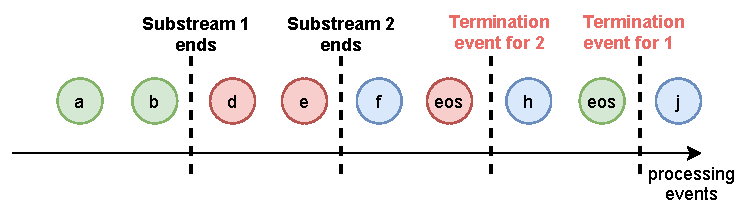
\includegraphics[width=0.80\textwidth]{Chapters/SubstreamConsistency/pics/notifications-reordering.pdf}
  \caption{An example of termination events reordering}
  \label{notifications_reordering}
\end{figure}

\begin{definition}[Consistent events order]
Let $e^{*}_1$ and $e^{*}_2$ be the last elements of substreams defined by predicates $Pred_1$ and $Pred_2$. Termination events $\langle eoss, p, Pred_1\rangle$ and $\langle eoss, p, Pred_2\rangle$ are {\em consistently ordered} iff:

\begin{equation}
e^{*}_1 >_p e^{*}_2 \Leftrightarrow \langle eoss, p, Pred_1\rangle >_p \langle eoss, p, Pred_2\rangle
\end{equation}
\end{definition}
